\chapter{General Methodology}\label{ch: general methodology}

This chapter describes the general methods that were applied in the long-read sequencing experiments in \textbf{Chapters 4 and 6}. Experimental methods specific to individual results chapters can be found in the Methods section of the relevant chapter. Methods pertaining to the library preparation for PacBio Isoform Sequencing (Iso-Seq) and ONT nanopore cDNA sequencing can be found in \cref{chap:isoseq_labpipeline} and \cref{chap:ont_labpipeline}, respectively. Standard manufacturer's protocols used in this thesis can be found in \textbf{Appendix \ref{app_longread_protocol} and \ref{app_longread_ont_protocol}}. All reagents mentioned in this Chapter were provided with the respective kits unless otherwise stated.

\section{Mouse tissue samples \& RNA Isolation}

\subsection{Mouse model of AD tauopathy: rTg4510} 
\label{ch2: rtg4510}
rTg4510 mice recapitulate AD tauopathy through the overexpression of the human tau transgene, MAPT\textsuperscript{P301L}, which harbours the FTD-associated P301L mutation. It contains four microtubule-binding domains while lacking the N-terminal segment (0N4R), and exons 2-3 of the mouse prion protein gene \textit{Prnp}. The transgene expression is controlled under the calcium calmodulin kinase II promoter (CaMK2a) and is largely restricted to the forebrain, with rapid age-dependent spread of neuropathology starting from as early as 2 months in the neocortex to the hippocampus by 5 months (\cref{fig:immunohistochemistry}). Neuronal and synaptic loss are also observed from 9 months, with these mice exhibiting cognitive and behavioural impairments. Sex differences in pathology have been reported with female mice exhibiting earlier and more severe cognitive and behavioural impairments than transgenic male mice\cite{M2011}. 

The rTg4510 mouse model is particularly informative as tau expression can be induced through the tetracycline operon-responsive element and suppressed upon doxycycline treatment\cite{Ramsden2005}. However, a recent study reported disruption of several endogenous mouse genes due to the random integration of MAPT\textsuperscript{P301L}, which has additional off-target effects that may potentially contribute to the neurodegenerative phenotype associated with rTg4510 transgenic mice\cite{Gamache2019}. 
 

\subsection{Animal breeding \& Sample Preparation}
\label{sec: animalbreeding_sample preparation}
All animal procedures were carried out at Eli Lilly and Company (Windlesham, UK), in accordance with the UK Animals (Scientific Procedures) Act 1986 and with approval of the local Animal Welfare and Ethical Review Board. The mice were housed under standard conditions (constant temperature and humidity with a 12h light/dark cycle in individually ventilated cages) before terminal anaesthesia with pentobarbital and transcardial perfusion with phosphate-buffered saline (PBS)\cite{Castanho2020}.

The entorhinal cortex was dissected from the left-brain hemisphere of female transgenic mice (TG\nomenclature{TG}{Transgenic mice}) and wild-type controls (WT\nomenclature{WT}{Wild-type mice}), aged 2, 4, 6 and 8 months (n = 9 - 10 mice per group). Total RNA was then extracted\cite{Castanho2020} using the AllPrep DNA/RNA Mini Kit (Qiagen) according to the manufacturer's protocol, and converted to cDNA for library preparation (described later in \cref{section:ch2_cDNA_synthesis_explanation}). Of note, more than 80\% of total RNA is comprised of ribosomal RNA (rRNA), with the remaining 15\% representing transfer RNA (tRNA) and only 1-5\% representing mRNA. 

\begin{landscape}
	\begin{figure}[htp]
		\centering
		\vspace{20pt}
		\includegraphics[page=3,trim={0 7cm 0 0 },clip, scale = 0.7]{Figures/Introduction_Figures_Landscape.pdf}
		\captionsetup{width=1.5\textwidth}
		\caption[Progressive pathological characterisation of rTg4510 mouse model]%
		{\textbf{Progressive pathological characterisation of rTg4510 mouse model.} Shown are \textbf{(A)} representative immunohistochemistry images from the hippocampus showing accumulation of tau in rTg4510 transgenic (TG) mice compared with wild-type (WT) mice at 2, 4, 6 and 8 months of age. \textbf{(B)} Progressive accumulation of tau is observed in the hippocampus and the \textbf{(C)} entorhinal cortex in rTg4510 TG but not WT mice. Figures and legends are adapted from Castanho et al. 2020 \cite{Castanho2020}.}
		\label{fig:immunohistochemistry}
	\end{figure}	
\end{landscape}

\subsection{Assessment of nucleic acid quality and quantity}
Acquiring high-quality RNA, generating full-length cDNA and successfully performing the multi-step library preparation are all crucial for optimal sequencing experiments, particularly long-read sequencing. The assessment of the purity and integrity of extracted RNA, followed by cDNA quality and quantity, was therefore required throughout library preparation and quality control (QC)\nomenclature{QC}{Quality control} stages of my sequencing experiments. This was undertaken using the RNA/DNA ScreenTape and Bioanalyzer assays for qualitative assessment, and the Qubit for DNA quantification. 


\subsection{ScreenTape \& Bioanalyzer assays}
\label{section:ch2_bioanalyzer} 
ScreenTape and Bioanalyzer assays are commonly used to provide an accurate and automated assessment of nucleic acid quality and size by electrophoresis. It works on the principle that upon applying an electric field, negatively-charged DNA migrates through a gel matrix towards the positive anode at a rate that is dependent on DNA size; smaller DNA fragments migrate faster, and thus move further through the gel within a specific time frame. The separated DNA can be then visualised using a fluorescent dye that intercalates into the double-stranded DNA (dsDNA\nomenclature{dsDNA}{Double-stranded DNA}) structure and fluoresces under ultraviolet light. 

Both RNA ScreenTape and Bioanalyzer assays further provide a numeric evaluation of the quality of an RNA sample using a score between 1 and 10, known as a RNA integrity number (RIN\nomenclature{RIN}{RNA integrity number}); a RIN score of 1 is indicative of high degradation and poor quality RNA, whereas a RIN score of 10 indicates minimal degradation (\cref{fig:bionalayzer_pics}). The purity and quantity of extracted RNA was assessed using the RNA Bioanalyzer assay with Agilent RNA 6000 Nano Kit (Agilent Technologies) and Agilent 2100 Bioanalyzer instrument (Agilent Technologies). 

Assessment of cDNA quality during various QC stages of long-read library preparation was mostly performed using the DNA Bioanalyzer assay with Agilent D1200 Kit (Agilent Technologies), particularly where accurate determination of library molarity was critical (given that the Bioanalyzer assay is more sensitive than the ScreenTape assay). However in QC stages where assessment is optional, the D5000 ScreenTape (Agilent Technologies) and 4200 TapeStation (Agilent Technologies) were used instead as the ScreenTape assay was most cost-effective and less time-consuming to run. Both assays were performed following the standard manufacturer's protocol. Briefly, this involved mixing the sample with the ladder and buffer (if using the ScreenTape), or with the marker and gel-dye mix (if using the Bioanalyzer assay), before loading the sample into the machine to be assayed. Detailed lab instructions for Bioanalyzer and ScreenTape assays are detailed in \textbf{Appendix \ref{Isoseq_Protocol_tapestation_bioanalyzer}}.

\subsection{Qubit}
\label{section:ch2_qubit}   
Qubit assays (Invitrogen) allow accurate nucleic acid quantification by the selective binding of fluorescent Qubit dyes to dsDNA or RNA, rendering it more sensitive and specific than the NanoDrop 8000 spectrophotometer (Thermo Fisher Scientific) which uses UV absorbance. Following RNA extraction, the RNA concentration was determined using Qubit assays to ensure that the same amount of total RNA for each sample was used for library preparation. Many of the QC steps post DNA purification (later discussed in \cref{section:ch2_AMPure_explanation}) throughout library preparation also required Qubit assays to determine the cDNA concentration prior to proceeding with downstream experiments. Briefly, this involved running two "standard samples" prepared with Qubit reagent in 10:200 ratio, and the "test samples" prepared with the same reagent in a 1:200 ratio, on the Qubit 3.0 Fluorometer (Thermo Fisher Scientific) following the standard manufacturer's protocol (detailed in \textbf{Appendix  \ref{Isoseq_Protocol_qubit}}). Of note, all quantity assessments in this thesis were performed using the Qubit DNA High sensitivity assay.          

\begin{figure}[htp]
	\centering
	\vspace{20pt}
	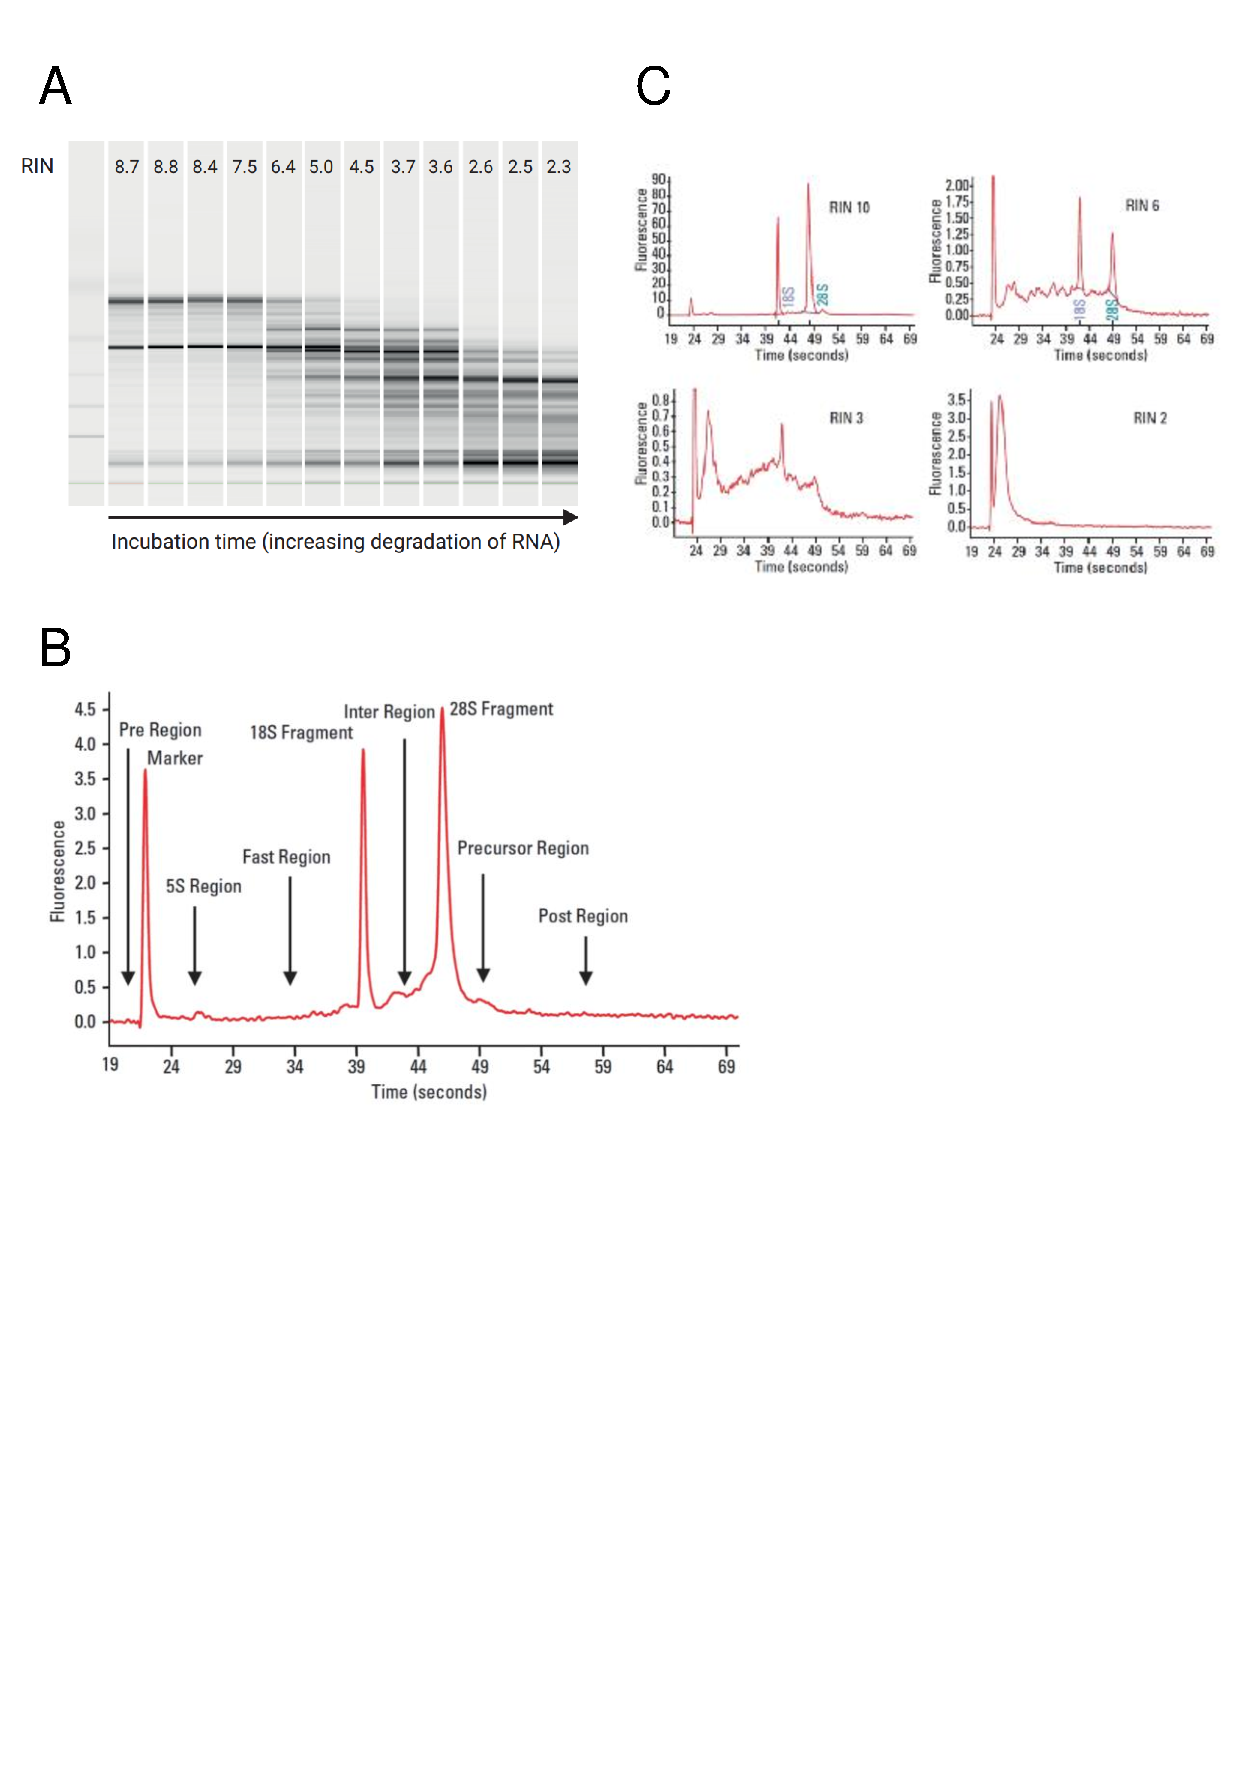
\includegraphics[page=1,trim={0 10cm 0 0 },clip, scale = 0.7]{Figures/General_Methodology_Figures.pdf}
	\captionsetup{width=0.95\textwidth}
	\caption[Evaluation of RNA integrity using ScreenTape \& Bioanalyzer assays]%
	{\textbf{Evaluation of RNA integrity using ScreenTape \& Bioanalyzer assays.} Shown is a \textbf{(A)} gel image from a Bioanalyzer assay demonstrating progressive total RNA degradation over a prolonged period of incubation. Degradation is indicated by a general shift to the right with more bands representing shorter fragments and a decrease in RIN. \textbf{(B)} An alternative assessment of total RNA quality and integrity is represented with the Bioanalyzer electropherogram with two distinctive peaks corresponding to 18S and 28S fragment of rRNA, and a marker peak. The RIN is calculated using the relative ratio of the Fast Region and 18S, 28S fragment. \textbf{(C)} Bioanalyzer electropherograms depicting total RNA with varying degrees of degradation: i) minimal (RIN = 10) as indicated by the two distinct peaks corresponding to 18S and 28S, ii) small degree (RIN = 6) with the two peaks still visible but also detection of other smaller peaks, corresponding to fragmented RNA, iii) large degree of degradation (RIN = 3) with inability to detect the two peaks, and iv) significant degradation (RIN = 2), indicated by the lack of large fragments. Figures and legends are adapted from Mueller et al. (2004)\cite{Mueller}.}
	\label{fig:bionalayzer_pics}
\end{figure}

\newpage
\section{cDNA synthesis, amplification \& purification}
After RNA isolation, integrity assessment and quantification, total RNA was converted to cDNA. Given the low frequency of mRNA (< 5\% of total RNA) and low sensitivity of current sequencing platforms, the converted cDNA was subsequently amplified using polymerase chain reaction (PCR\nomenclature{PCR}{Polymerase chain reaction}) and assessed using agarose gel electrophoresis. 


\subsection{Complementary DNA synthesis}
\label{section:ch2_cDNA_synthesis_explanation} 
Recommended as part of the Iso-Seq protocol, the SMARTer PCR cDNA Synthesis Kit (Clontech) was used to convert 200ng total RNA to cDNA. Unlike other cDNA synthesis methods, the SMARTer PCR cDNA synthesis relies on a modified oligo(dT) primer and a reverse transcriptase (RT\nomenclature{RT}{Reverse transcriptase}) that has an inherent terminal transferase activity (outlined in \cref{fig:cDNAsynthesis_workflow}). First-strand synthesis therefore occurs in a SMART (\underline{S}witching \underline{M}echanism \underline{A}t 5' End of \underline{R}NA \underline{T}ranscript) fashion, whereby a few additional nucleotides ("overhang") are added to the 3' end of the cDNA as the RT approaches the 5' end of the mRNA. The RT then switches templates and continues replicating to the end, generating a full-length single-stranded cDNA which is then amplified. The usage of the "overhang" sequence ensured enrichment and synthesis of full-length cDNA, as cDNA without this sequence (i.e. prematurely terminated cDNA, cDNA from non-poly(A) RNA, contaminating genomic DNA) will not be exponentially amplified \cite{Ramskold2012}. Detailed manufacturer's instructions of this kit can be found in \textbf{Appendix \ref{Isoseq_protocol_cDNAsynthesis}}. 

While this kit is advantageous in preferentially enriching for full-length cDNA sequences, it cannot differentiate between intact and truncated RNA, which is present in poor-quality samples and could be amplified as technical artefacts in the final cDNA library. A solution to circumvent this issue is to exploit the the presence of the 5’-cap which is only present in intact RNA (5'-cap refers to 7-methylguanosine at the 5’ end of mRNA which is added during transcription to protect nascent mRNA from degradation and assist in protein translation), using the Full-Length cDNA Amplification kit (Teloprime)\cite{Cartolano2016}. This kit relies on a double-stranded adapter that recognises and ligates to the 5’ cap at the end of the first-strand synthesis step. I trialled this kit as part of my experiments, but was unable to generate sufficient cDNA. 

\begin{figure}[htp]
	\centering
	\vspace{20pt}
	\includegraphics[page=2,trim={0 12cm 0 0 },clip, scale = 0.7]{Figures/General_Methodology_Figures.pdf}
	\captionsetup{width=0.95\textwidth,singlelinecheck=off}
	\caption[SMARTer cDNA synthesis]%
	{\textbf{SMARTer cDNA synthesis.} Shown is a flowchart of the SMARTer cDNA synthesis protocol to ensure the generation of full-length cDNA by leveraging the power of the enzyme's terminal transferase activity. Premature RT termination reduces the efficiency of the transferase activity, resulting in the absence of the overhang at the 3' end of the template for downstream amplification. 
	cDNA synthesis is achieved in the following manner: 
	\begin{enumerate}
		\item Oligo(dT) primer (3’ SMART CDS Primer II A) primes the first-strand synthesis reaction by binding to the poly(A) tail and transcribes the RNA into single-stranded DNA.
		\item As RT reaches the 5’ end of the mRNA, the enzyme’s terminal transferase activity adds a few additional nucleotides to the 3’ end of the cDNA.
		\item With a 3’ end that is complementary to the added nucleotides, the SMARTer II A oligonucleotide (or the template switching oligonucleotide) base-pairs with it and creates an extended template.
		\item RT then switches templates and continues transcribing to the end of the SMARTer oligonucleotide. 
		\item The resulting full-length, single-stranded cDNA contains the complete 5’ end of the mRNA, as well as a 3’ end that is complementary to the SMARTer oligonucleotide. 
		\item The SMARTer oligonucleotide and the poly(A) sequence then serve as universal priming sites for end-to-end cDNA amplification.
		\\
		
	\end{enumerate}
	Of note, the SMARTer II A Oligonucleotide, 3’ SMART CDS Primer II A, and 5’ PCR Primer II A all contain a stretch of identical sequence.  

	Figure and legend are taken from the SMARTer PCR cDNA Synthesis Kit User Manual\cite{LaboratoriesInc}. RT - Reverse transcriptase.
	}
	\label{fig:cDNAsynthesis_workflow}
\end{figure}

\clearpage
To maximise throughput and minimise cost, my targeted experiments (\textbf{Chapters 6}) involved sequencing of multiple samples simultaneously in one sequencing run (i.e. in “multiplex”). To differentiate the samples, I used a unique barcoded oligo(dT) primer (\cref{tab:barcode_primers}) for each sample for cDNA synthesis instead of the standard oligo(dT) primer from the SMARTer cDNA synthesis kit (Clontech). The only difference between the barcoded oligo(dT) and the standard oligo(dT) primer is the addition of a unique 16-bp internal barcode, which does not interfere with priming and end-to-end cDNA amplification. The general structure of the barcoded oligo(dT) primer were as follows:

\vspace{0.5cm}
%\hspace{5cm} \textcolor{RedOrange}{Primer Sequence} \hspace{2cm}   \textcolor{ForestGreen}{16-bp barcode}   \hspace{2cm} \textcolor{RoyalBlue}{oligo(dT)}
\hspace{2cm} \textcolor{RedOrange}{Primer sequence} \hspace{0.8cm}   \textcolor{ForestGreen}{16bp barcode}   \hspace{3cm} \textcolor{RoyalBlue}{oligo(dT)}
\vspace{-1.2cm}
\begin{center}
	\footnotesize{5'\textcolor{RedOrange}{AAGCAGTGGTATCAACGCAGAGTAC}\textcolor{ForestGreen}{tcagacgatgcgtcat}\textcolor{RoyalBlue}{TTTTTTTTTTTTTTTTTTTTTTTTTTTTTTVN}3’}
\end{center}

\begin{landscape}
	\begin{table}[ht]
		\centering
		\captionsetup{width=1.5\textwidth}
		\caption[Barcoded oligo(dT) primers for targeted profiling]%
		{\textbf{Barcoded oligo(dT) primers were used for multiplexing samples in targeted profiling.} Tabulated is a list of barcoded primers that were used for targeted profiling of AD-risk genes in the rTg4510 cortex. Each of the barcoded primers contain the same 5' primer sequence and oligo(dT) for reverse transcription of first-strand cDNA synthesis using the SMARTer PCR cDNA Synthesis Kit (Clontech). The barcodes were provided from the official PacBio multiplex protocol.}
		\label{tab:barcode_primers}
		\vspace{1cm}
		\begin{tabularx}{1.5\textwidth}{cc}
			\toprule
			Barcode & Sequence                                                                  \\ \midrule
			Barcode 1    & AAGCAGTGGTATCAACGCAGAGTACCACATATCAGAGTGCGTTTTTTTTTTTTTTTTTTTTTTTTTTTTTTVN \\
			Barcode 2    & AAGCAGTGGTATCAACGCAGAGTACACACACAGACTGTGAGTTTTTTTTTTTTTTTTTTTTTTTTTTTTTTVN \\
			Barcode 3    & AAGCAGTGGTATCAACGCAGAGTACACACATCTCGTGAGAGTTTTTTTTTTTTTTTTTTTTTTTTTTTTTTVN \\
			Barcode 4    & AAGCAGTGGTATCAACGCAGAGTACCACGCACACACGCGCGTTTTTTTTTTTTTTTTTTTTTTTTTTTTTTVN \\
			Barcode 5    & AAGCAGTGGTATCAACGCAGAGTACCACTCGACTCTCGCGTTTTTTTTTTTTTTTTTTTTTTTTTTTTTTTVN \\
			Barcode 6    & AAGCAGTGGTATCAACGCAGAGTACCATATATATCAGCTGTTTTTTTTTTTTTTTTTTTTTTTTTTTTTTTVN \\
			Barcode 7    & AAGCAGTGGTATCAACGCAGAGTACTCTGTATCTCTATGTGTTTTTTTTTTTTTTTTTTTTTTTTTTTTTTVN \\
			Barcode 8    & AAGCAGTGGTATCAACGCAGAGTACACAGTCGAGCGCTGCGTTTTTTTTTTTTTTTTTTTTTTTTTTTTTTVN \\
			Barcode 9    & AAGCAGTGGTATCAACGCAGAGTACACACACGCGAGACAGATTTTTTTTTTTTTTTTTTTTTTTTTTTTTTVN \\
			Barcode 10 & AAGCAGTGGTATCAACGCAGAGTACACGCGCTATCTCAGAGTTTTTTTTTTTTTTTTTTTTTTTTTTTTTTVN \\ \bottomrule
		\end{tabularx}
	\end{table}
\end{landscape}


\subsection{Polymerase Chain Reaction (PCR)}
\label{section:ch2_PCR_explanation} 
The PCR is a well-established method for generating multiple copies of the same DNA sequence. Mimicking natural DNA replication, this relies on a thermostable DNA polymerase, a set of primers specific to the region of interest, and a cocktail of reagents required for polymerisation (i.e. deoxynucleotides (dNTPs)\nomenclature{dNTPs}{Deoxynucleotide triphosphates} and buffers). This reaction is subjected to a series of heating and cooling steps: 
\begin{enumerate}
	\item Denaturation at 96$^{\circ}$C to separate dsDNA. 
	\item Annealing, typically between 55$^{\circ}$C  and 65$^{\circ}$C, for the binding of primers to the complementary sequences on the single-stranded DNA; the specific annealing temperature is dependent on the primer sequence. 
	\item Extension at 72$^{\circ}$C to allow the polymerase to extend the primers, synthesising a new cDNA strand using dNTPs.
\end{enumerate} 
These three steps are then repeated multiple times, or "cycles", resulting in an exponential generation of the DNA template of interest.

\subsection{Agarose Gel Electrophoresis}
\label{section:ch2_agarose_explanation}  
Agarose gel electrophoresis allows the separation of dsDNA molecules based on length, and works on the same principle as the Bioanalyzer and ScreenTape assays (described previously in \cref{section:ch2_bioanalyzer}). It is most commonly used to determine DNA quality and quantity, and assess the efficiency of molecular biology techniques such as PCR amplification by determining the number of optimal cycles. It is a well known phenomenon that an increased number of unnecessary PCR cycles can generate artefacts (strand invasion) and preferentially amplify shorter transcripts\cite{Acinas2005,Bayega2018}. Instructions to prepare and run an agarose gel electrophoresis are detailed in \textbf{Appendix \ref{Isoseq_Protocol_running_agarose_gel}}.


\subsection{AMPure bead Purification} 
\label{section:ch2_AMPure_explanation} 
At various stages of long-read library preparation, cDNA was purified using AMPure beads (\cref{fig:ampure_bead_workflow}\textbf{A}). These are paramagnetic beads that reversibly bind to DNA in the presence of polyethylene glycol (PEG) and salt. The concentration of PEG, and consequent ratio of beads to DNA, determines the size of fragments that are bound and subsequently eluted (\cref{fig:ampure_bead_workflow}\textbf{B}); the lower the concentration of beads to DNA, the greater the proportion of longer DNA fragments bound, due to the preferential binding of beads to larger molecular weight DNA with a higher negative charge - a 0.4X ratio would therefore preferentially retain the larger DNA fragments, whereas a 1X ratio would retain both long and short DNA fragments (\cref{fig:ampure_bead_workflow}\textbf{B}). Briefly, AMPure bead purification was performed by thoroughly mixing and vortexing each sample with a pre-specified ratio of AMPure beads. The samples were then placed onto a magnet for clear separation of DNA-bound beads and solution, followed by two washes of 70\% ethanol and DNA elution. Detailed instructions can be found in \cref{general_ampure_bead_purification}.

\begin{figure}[!h]
	\centering
	\includegraphics[page=3,trim={0 8cm 0 0cm},clip, scale = 0.7]{Figures/General_Methodology_Figures.pdf}
	\captionsetup{width=0.95\textwidth}
	\caption[cDNA purification with AMPure beads]%
	{\textbf{cDNA purification with AMPure beads.} Shown is a schematic figure depicting the \textbf{(A)} steps of purifying DNA with AMPure beads, with initial binding of magnetic beads to negatively-charged DNA, followed by ethanol wash and elution. \textbf{(B)}) An agarose gel image of DNA purified using a range of bead to DNA ratio for size selection; the lower the ratio, the greater the enrichment for longer fragments with displacement of the shorter fragments. Figures are taken from the Beckman website.}
	\label{fig:ampure_bead_workflow}
\end{figure}

\clearpage
\section{ERCC-RNA Spike-In Controls}
\label{section:ch2_ERCC_explanation} 
A set of external RNA Spike-In controls, generated by the External RNA Controls Consortium (hereby referred to as "ERCC"\nomenclature{ERCC}{External RNA Controls Consortium}), was used to i) evaluate the performance of library preparation and the sequencing experiments, and to ii) validate the Iso-Seq bioinformatics pipeline in accurately characterising the transcriptome using long reads. ERCC consists of 92 polyadenylated synthetic transcripts (250 to 2000 nucleotides) of known sequences from the ERCC plasmid library, which were added in pre-determined amounts to the sample before first-strand cDNA synthesis. The usage of ERCC allowed me to assess the quantitative power of long-read sequencing in addition to providing absolute quantification of mRNA isoforms (with the generation of a standard curve). It can further assess the validity of the bioinformatic analysis as only one unique molecule per ERCC should be detected. 

The amount of ERCC added was determined using the below equation \cite{WTAC}:
\begin{myequation}[!h]
	\label{eqn:ercc_calcaluations}
	\begin{equation*}
		mass_{RNA spike} = fraction_{spiked reads}\; * fraction_{target RNA}\; *mass_{RNA input}
	\end{equation*}
	\begin{equation*}
		concentration_{RNA spike} = mass_{RNA spike}\; * volume_{RNA spike}
	\end{equation*}
	where:
	\begin{conditions*}
		mass_{RNA spike} & mass of ERCC to be added to sample \\
		concentration_{RNA spike} & final diluted concentration (ng/$\mu$l) of ERCC \\
		fraction_{spiked reads}  &   desired proportion of sequenced ERCC reads relative to total amount of sequenced reads \textit{(3\%)} \\
		fraction_{target RNA}    &  expected proportion of target RNA, in this case mRNA relative to total RNA \textit{(3\%)} \\   
		mass_{RNA input} &  input of total RNA \textit{(200ng)} \\
		volume_{RNA spike} & volume of RNA spike-in \textit{(0.1$\mu$L)}				
	\end{conditions*}
	\captionsetup{width=0.95\textwidth}
	\caption[Determining the amount of ERCC controls for sequencing runs]%
	{\textbf{Determining the amount of ERCC controls for sequencing runs.} In determining the mass and final concentration of RNA-spike-in mix based on the above conditions, the stock ERCC RNA spike-in was diluted from the original concentration of 30ng/$\mu$L to 1.8ng/$\mu$L with a dilution factor of 1:16.8. The italicised parameters were taken from the "Wellcome Trust Advanced Course: RNA Transcriptomics (2018)"\cite{WTAC} (that I attended during my PhD) with the exception of total RNA input.}
\end{myequation}

A separate pilot experiment (\textbf{Appendix \ref{ch:alt_cDNA}}) showed successful addition of ERCC with two main bands at \textasciitilde600bp and \textasciitilde1000bp (\cref{fig:ercc_lab_gel}\textbf{A}), reflecting significant enrichment of ERCC at these two respective lengths as expected (\cref{fig:ercc_lab_gel}\textbf{B}). However, the stark contrast of these two bands against the smear of cDNA suggests over-usage of ERCC - possibly due to the overestimation of assumed proportion of mRNA. A lower ERCC amount was therefore used across all the experiments to reduce unnecessary sequencing and coverage of ERCC (final concentration of 0.6ng/$\mu$L with a dilution factor of 1:50.5, \cref{fig:ercc_lab_gel}\textbf{C}). 

\vspace{1cm}
\begin{figure}[!htp]
	\begin{center}
		\includegraphics[page=4,trim={0 8cm 0 1cm},clip,scale = 0.65]{Figures/General_Methodology_Figures.pdf}
	\end{center}
	\captionsetup{width=0.95\textwidth}
	\caption[Usage of ERCC controls to evaluate performance of long-read sequencing runs]%
	{\textbf{Usage of ERCC controls to evaluate performance of long-read sequencing runs.} Shown is \textbf{(A)} an agarose gel image taken from PCR amplification of cDNA and ERCC (1.8ng/$\mu$L determined from \textbf{Equation 2.1}), and ERCC alone as a positive control. 5$\mu$L of PCR aliquots were taken every cycle (cycles 13 to 18) and then assessed on gel electrophoresis. The two bands at 600bp and 1000bp correspond to the enrichment of ERCC at these two lengths as expected. \textbf{(B)} Distribution of known ERCC length, with a significant proportion of transcripts sized at 500-600bp and 1000-1200bp. \textbf{(C)} An agarose gel image after a repeat of PCR amplification of cDNA and ERCC at a lower concentration (0.6ng/$\mu$L) with ERCC as positive and water as negative control, respectively. The numbers above the lanes refer to the number of PCR cycles. L denotes to 100bp Ladder.}
	\label{fig:ercc_lab_gel}
\end{figure}
 
